\documentclass[10pt]{beamer}

\usetheme[progressbar=frametitle]{metropolis}
\usecolortheme{wolf}
\usepackage{appendixnumberbeamer}
\usepackage{tikz}
\usetikzlibrary{arrows.meta, positioning, quotes}


\usepackage{booktabs}
\usepackage[scale=2]{ccicons}

\usepackage{pgfplots}
\usepgfplotslibrary{dateplot}

\usepackage{xspace}
\newcommand{\themename}{\textbf{\textsc{metropolis}}\xspace}
\def\SNATopicTH{พฤติกรรมของผู้เรียนในระบบการเรียนออนไลน์ขนาดใหญ่ ซึ่งนำไปสู่การยุติการเรียน}
\def\SNATopicEN{Behavior of Online Learner in MOOC Platform Leading to Course Drop-out}

\title{\SNATopicEN}
\subtitle{Project Structure, Features and Model}
\author{Sitdhibong Laokok}
\institute{Srinakharinwirot University}
\titlegraphic{%
    
\includegraphics[width=.15\textwidth]{Srinakharinwirot_Logo_EN_Color.png}\hfill
}

\makeatletter
\setbeamertemplate{title page}{
  \begin{minipage}[b][\paperheight]{\textwidth}
    \vfill%
    \ifx\inserttitle\@empty\else\usebeamertemplate*{title}\fi
    \ifx\insertsubtitle\@empty\else\usebeamertemplate*{subtitle}\fi
    \usebeamertemplate*{title separator}
    \ifx\beamer@shortauthor\@empty\else\usebeamertemplate*{author}\fi
    \ifx\insertdate\@empty\else\usebeamertemplate*{date}\fi
    \ifx\insertinstitute\@empty\else\usebeamertemplate*{institute}\fi
    \vfill
    \ifx\inserttitlegraphic\@empty\else\inserttitlegraphic\fi
    \vspace*{1cm}
  \end{minipage}
}
\makeatother

\begin{document}
    \begin{frame}
        \titlepage
    \end{frame}

    \section[Dataset]{Dataset}
    \begin{frame}[fragile]{Dataset}
        This dataset has information collected from learner in MOOC platform with
        course information, enrollment, learner's course paticipations,
        and enrollment labelling for indicates drop-out status. 
        The dataset separated in to 4 files to contain an information above.
    \end{frame}

    \section[Dataset Description]{Dataset Description}
    \begin{frame}[fragile]{Course Information}
        Each line contain the timespan of each course in logged information. 
        The timespan of each course for calculating dropouts is 10 days after the last day of the course, i.e.,
        course C if from 01/04/2014 to 30/04/2014 in the given data, 
        a user enrolled the corse C will be treated as a drop-out if he/she leaves no record from 01/05/2015 to 10/05/2014.
        \begin{table}
            \caption{\label{tab:course-info}Course's timespan}
            \begin{tabular}{l*{2}{l}r}
                Field name  & Description \\
                \hline
                course\_id  & Course id \\
                from        & The first day of the course in log \\
                to          & The last day of the course in log \\
            \end{tabular}
        \end{table}

    \end{frame}

    \begin{frame}{Course Information}
        each line in this file describes a module in a course with its category, 
        children objects and release time. Those modules represent different 
        online materials of the courses, e.g., chapters, videos, problem sets 
        and etc. The modules are organized as a tree, i.e., 
        each course contains several chapters; each chapter contains several 
        sections; and each section contains several objects 
        (videos, problem sets, and etc).

        \begin{table}
            \caption{\label{tab:course-object}Course's object}
            \begin{tabular}{l*{2}{l}r}
                Field name  & Description \\
                \hline
                course\_id  & Course id \\
                module\_id  & The ID of a course module \\
                category    & The category of the course module \\
                children    & The children modules of the course module \\
                start       & The time that the module was released to students \\
            \end{tabular}
        \end{table}
    \end{frame}

    \begin{frame}[fragile]{Course Enrollment}
        Each line is a course enrollment record with an enrollment id, 
        a username U and a course id C, indicating that U enrolled in course C.

        \begin{table}
            \caption{\label{tab:course-enrollment}Course Enrollment Information}
            \begin{tabular}{l*{2}{l}r}
                Field name      & Description \\
                \hline
                enrollment\_id  & Enrollment ID \\
                username        & Student ID \\
                course\_id      & Course ID \\
            \end{tabular}
        \end{table}
    \end{frame}

    \begin{frame}[fragile]{Course Action Logs}
        Each line is a behavior record. Each event contains the following 
        information: enrollment\_id, username, course\_id, time, 
        source (server or browser), event, and object. 

        \begin{table}
            \caption{\label{tab:course-action-logs}Action Logs}
            \begin{tabular}{l*{2}{l}r}
                Field name      & Description \\
                \hline
                enrollment\_id  & Enrollment ID \\
                username        & Time of the event \\
                source          & Event source (Server or Browser) \\
                event           & In terms of event type, there are 7 different event types \\
                object          & The object the student access or navigate to \\
            \end{tabular}
        \end{table}
    \end{frame}

    \begin{frame}[fragile]{Event meaning}
        From Table \ref{tab:course-action-logs}, There are 7 type fo event collected
        from learner's participation in course. All possible values are shown in 
        Table \ref{tab:event-meaning}
        \begin{table}
            \caption{\label{tab:event-meaning}Events}
            \begin{tabular}{l*{2}{l}r}
                Event Id        & Description \\
                \hline
                1               & \textbf{Problem}: Working on course assignments \\
                2               & \textbf{Video}: Watching course videos \\
                3               & \textbf{Access}: Accessing other courseobject except videos and assignments \\
                4               & \textbf{Wiki}: Accessing the course wiki \\
                5               & \textbf{Discussion}: Access the course forum \\
                6               & \textbf{Navigate}:  Navigating to the part of the course \\
                7               & \textbf{Page close}:  Closing the web page \\
            \end{tabular}
        \end{table}
    \end{frame}

    \begin{frame}{Enrollment Labelling}
        Each line contains information about the ground truth of enrollments 
        in the training set. 

        \begin{table}
            \caption{\label{tab:course-dropped-out-indicator}Enrollment Labelling}
            \begin{tabular}{l*{2}{l}r}
                Field name      & Description \\
                \hline
                enrollment\_id  & Enrollment ID \\
                status          & Study status 1 for dropped-out, 2 for otherwise  \\
            \end{tabular}
        \end{table}
    \end{frame}

    \section[Data Modeling]{Data Modeling}
    \begin{frame}[fragile]{Data Modeling}
        \begin{figure}
            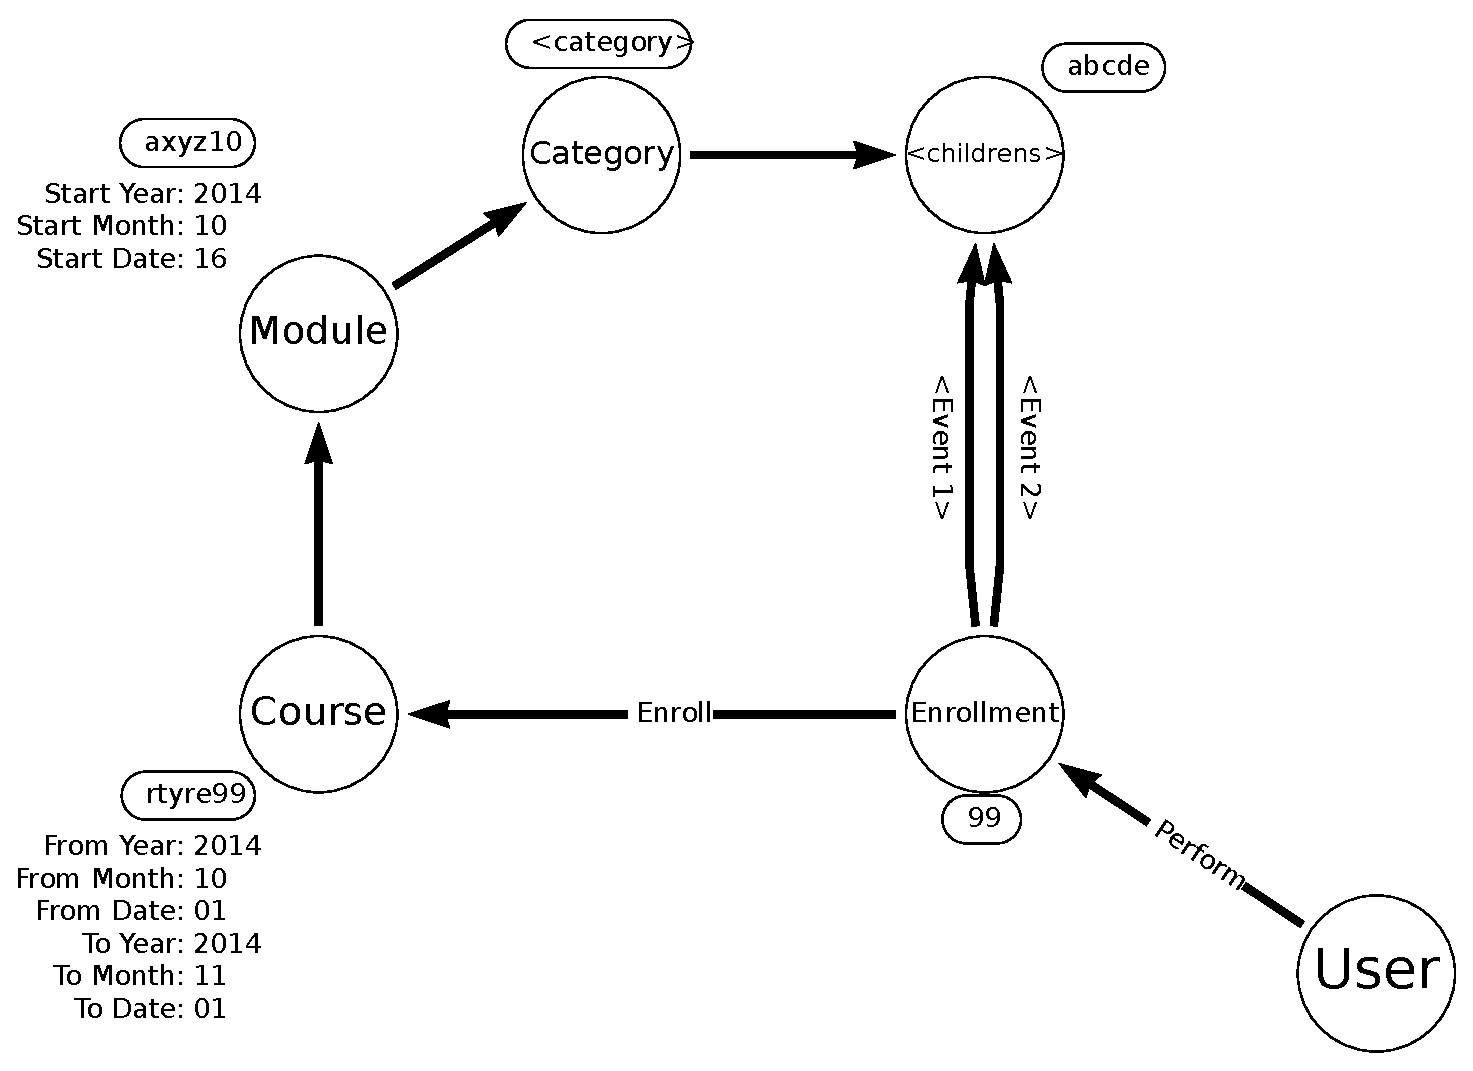
\includegraphics[width=0.9\textwidth]{asset/action-structure.eps}
            \caption{\label{fig:model-structure}Data model}
        \end{figure}
    \end{frame}
\end{document}